\cotefile{81}
\scanpage{2}
\unsure{0|O}\quad Cartes sphériques en général
% archive sheet number: 1

\scanpage{3}
Carte sphérique \inserted{(orientée)} avec repère (dans cat. \unsure{isotopiques|isotopique})

\[
\rotatebox{90}{$\simeq$}
\]
\unsure{morphisme|morphismes} $\mathbb P^{1}_{\mathbb C}\overset{f}{\unsure{-|\longrightarrow}}\mathbb P^{1}_{\mathrm C}$ ``spécial'' i.e
\[
 f(0)=0,\quad f(1)=1,\quad f(\infty)=\infty.\quad f\ \text{étale au dessus de }\mathbb P^{1}-\{0,1,\infty\}
\]
\[
\rotatebox{90}{$\simeq$}
\]
fonction rationnelle $f(z)$ telle que $f(0)=\deleted{\unsure{1}}0$, $f(1)=1$, $f(\infty)=\infty$ et telle que pour $z\in\mathbb C$ \deleted{telle que}\inserted{avec} $f(z)\deleted{\in}\notin\{0,\infty\}$ $f'(z)=0$, on ait $f(z)\deleted{\in}=1$ \deleted{\unsure{$\{0,1,\infty$}}$\}$ \inserted{et de plus} $f''(z)\ne0$ (i.e. la ramification de $f$ en $z$ est $2$)\ldots.

\[
\rotatebox{90}{$\simeq$}
\]
couple $P,Q$ \inserted{$[f=P/Q\quad !\,]$} de polynômes $\in\mathbb C(z)$ premiers entre eux \inserted{(i.e. sans zéros communs)} tels que $P(0)=0$, (donc $Q(0)\ne0$) $P(1)=Q(1)$ (donc $\ne0$), $\deg Q<\deg P$ (ces conditions expriment resp\textsuperscript{t} $f(0)=0$, $f(1)=1$, $f(\infty)=\infty$)
% slanted
\margin{On pourrait aussi normaliser \unsure{au lieu de cel|au lieu de cela} par $Q(0)=1$, ou $P$ unitaire, ou $Q$ unitaire\ldots}
normalisés (par exemple) par $P(1)=Q(1)=1$, et tels que pour $z\in\mathbb C$ avec $[f(z)\deleted{\in}\notin\{0,\infty\}, f'(z)=0,\ \mathrm{i.e.}\,]$ \inserted{$P(z)\ne0$,} $Q(z)\ne0$,
\[
 \frac{P'(z)\deleted{Q(z)}}{P(z)}-\frac{Q'(z)}{Q(z)}=0,
\]
on ait $P(z)=Q(z)$, et de plus
\[
 \frac{P''(z)}{P(z)}-\frac{Q''(z)}{Q(z)}\ne0\qquad\text{i.e.}\quad P''(z)\ne Q''(z)\ldots
\]
[ NB on a
\[
\begin{aligned}
 Q(z)P'(z)-P(z)Q'(z)&=\deleted{Q(z)[P'(z)-P(z)]+P(z)(Q(z)-Q'(z))}\\
 &\phantom{=}\inserted{(Q(z)-P(z))P'(z)+P(z)(P'(z)-Q'(z))}
\end{aligned}
\]
donc si \inserted{pour $P(z);Q(z)\ne0$} cette quantité est nulle, (i.e. $f'(z)=0$), alors $P(z)=Q(z)$ \deleted{\unsure{au|ou}} i.e $Q(z)-P(z)=0$ implique $P'(z)=Q'(z)$ et inversement si $P'(z)=Q'(z)$ on a $(Q(z)-P(z))P'(z)=0$ donc \uline{si} $P'(z)\ne0$, on a $P(z)=Q(z)$ ! Mais peut-on avoir $P'(z)=0$ (d'où aussi $Q'(z)=0$) \inserted{avec $P'(z)=Q'(z)$}\unsure{$\}$|)} sans avoir $P(z)=Q(z)$ ?

\deleted{\unsure{Réfléchissons} $Q(T)=$}

Prenons p.ex. $Q(T)=1$, les conditions sur $P$ deviennent $P(0)=0$, $P(1)=1$, $\deg P\geq1$ \inserted{(conséquence des deux précédentes)}, donc $P(T)=\unsure{T}P_0(T)$ où on a $P_0(1)=1$, la question devient si on peut avoir \inserted{(pour $P(z)\ne0$)} $P'(z)=0$ sans avoir $P(z)=1$ certes oui p.ex. $\deleted{P(T)=T^2}$ si $P(T)=T(aT+b)=aT^2+bT$, $a+b=1$, on a
% margin note written sideways
\margin{\raggedright $P'(T)=2aT+b$ qui est nul \inserted{(supposons $a\ne0$)} pour $z=-\frac{b}{2a}$ \deleted{\unsure{sera}} $\ne\left\{\begin{smallmatrix}0\\-\frac{b}{a}\end{smallmatrix}\right.$ \deleted{\illegible{1}} les deux zéros de $P$ si $b\ne0$, et $P(-\frac{b}{2a})=-\frac{b}{2a}(-\frac b2+b)=-\frac{b^2}{4a}$ qui \deleted{\unsure{peut être}} est $\ne1$ \deleted{\unsure{en prenant}} si $b^2\ne-4a$---}
% archive sheet number: 2

\scanpage{4}
% Whole-page cancellation: two long diagonal strokes cross the two columns.
% Local cancellations are nested inside the whole-page deletion state.
\[
\deleted{\begin{aligned}
 f_{d-2}e_1&=-e_{d-2}f_1\qquad(=\unsure{\eta|\gamma}_{d-1}\unsure{\}|\,}=\eta)\\
 \delta(\eta)&=e_{d-2}
\end{aligned}}
\]
\[
\deleted{\underline{\boxed{\begin{gathered}
(1\leq i\leq d-2)\\
\left\{\begin{aligned}
e_i e_1&=0\qquad f_i f_1=\begin{cases}0&\text{si }i\text{ impair}\\f_{i+1}&\text{si }i\text{ pair}\end{cases}\\
f_i e_1&=e_{i+1}\\
e_i f_1&=\begin{cases}-e_{i+1}&\text{si }i\text{ impair}\\0&\text{si }i\text{ pair}\end{cases}\qquad\unsure{\text{''}}
\end{aligned}\right.
\end{gathered}}}}
\]
% Two isolated quotation-like ticks stand at the right inside the box.
% A separate lower rule retraces the frame; the underline preserves the second lower stroke.
\[
\deleted{xf_1=f_1x=0\quad\text{si }\deg x\text{ pair}\qquad
 \eta=e_{d-1}\quad\delta(e_{d-1})=e_{d-2}}
\]
\[
\deleted{\unsure{\cdot}\quad\deleted{xf_1}}
\]
\[
\deleted{\begin{aligned}
 &(f_i+\lambda e_{\unsure{i|1}})(f_1+\lambda e_1)\\
 &=\underset{\inserted{f_{i+1}}}{\deleted{f_i f_1}}+\lambda^2\deleted{e_i e_1}
 +\lambda\bigl(\underbrace{f_i e_1}_{\inserted{e_{i+1}}}+
 \underbrace{\deleted{e_i f_1}}_{\inserted{\deleted{\unsure{-|\,}e_{i+1}}}}\bigr)
\end{aligned}}
\]
\[
\deleted{\begin{aligned}e_2&=f_1e_1\\e_3&=f_2e_1\end{aligned}}
\]
% margin note written upside down
\margin{\deleted{$\deleted{e_1 f_d}$}\quad
\deleted{$e_i e_1=0\qquad 1\leq i\leq d-2$}\quad
\deleted{$f_i f_1=$}}
\[
\deleted{\deleted{\delta(e_i e_j)=\unsure{0}}\qquad\delta(e_i e_j)=}
\]
\[
\deleted{\begin{gathered}
1\leq i\leq d-2\\
\left\{\begin{aligned}
e_i e_1&=0\\
f_i f_1&=\begin{cases}0&\text{si }i\text{ impair}\\ f_{i+1}&\text{si }i\text{ pair}\end{cases}\\
f_i e_1&=\eta_{i+1}=\alpha e_{i+1}+\beta f_{i+1}\\
e_i f_1&=\begin{cases}
\overset{\inserted{-}}{\deleted{\unsure{a|0}}}\eta_{i+1}=-\alpha e_{i+1}-\beta f_{i+1}&i\text{ impair}\\
-\eta_{i+1}+e_{i+1}=(1-\alpha)e_{i+1}-\beta f_{i+1}&i\text{ pair}
\end{cases}
\end{aligned}\right.
\end{gathered}}
\]
\[
\deleted{\underline{f_1e_1\deleted{f_1}=-e_1f_1=\eta_2=\alpha e_2+\beta f_2}}
\]
\[
\deleted{\begin{array}{c l}
1\leq i\leq d-3&\\
(e_i f_1)e_1&=\deleted{\unsure{-e_i}}
\begin{cases}
-\eta_{i+1}e_1=-\beta f_{i+1}e_1=-\beta\eta_{i+2}&i\text{ imp}\\
-\eta_{i-1}e_1+\deleted{e_{i+1}e_1}=-\beta\eta_{i+2}&i\text{ pair}
\end{cases}\\
\rotatebox{90}{$=$}&\\
e_i(f_1e_1)&\deleted{=e_i\eta_2=e_i(\alpha e_2+\beta\unsure{\bar f_2|\vec f_2|f_2})}\\
\rotatebox{90}{$=$}&\\
-e_i(e_1 f_1)&\\
\rotatebox{90}{$=$}&\\
-(e_i e_1)f_1=0&\text{donc}\quad
\tikz[baseline=(a.base)]\node[draw,circle,inner sep=1pt] (a) {$\beta=0$};\quad\alpha=\pm1
\end{array}}
\]
\[
\deleted{\text{donc}\quad\delta\eta=\pm e_{d-2}\qquad\unsure{Q\Phi S|QDS|QPS|QFS}}
\]
\[
\deleted{\begin{aligned}
\eta&=f_{d-2}e_1\\
\delta\eta&=\delta(f_{d-2})e_1=f_{d-3}e_1.
\end{aligned}}
\]
% Faint unassigned surface traces at lower right and above e_2 were inspected; no secure character was assigned.
% archive sheet number: 3

\scanpage{5}
\(\overset{\hspace{0.55em}\unsure{?}}{\text{\uline{NB}}}\)\quad Si $\sigma$ est un $\underset{\hspace{-1.3em}\unsure{\cdot}}{\text{automorphisme}}$ du corps des complexes, et si $f$ est ``spécial'', alors $f^\sigma$ est \unsure{égalmt|également} spécial -- donc $\operatorname{Aut}(\mathbb C)$ opere sur l'ens des $f$ spèciaux. Mais il opère par l'intermédiaire de $\operatorname{Aut}(\unsure{\overline{\mathrm Q}|\overline{\mathbb Q}})$, car si $f=P/Q$ spécial, les $\underset{\hspace{1.5em}\unsure{-|=}}{\text{coeff.}}$ de $P,Q$ sont des \uline{nbs algébriques}. Il revient au $=$ de dire que les zéros de $P,Q$ sont des nbs algébriques, i.e. le diviseur de $f$ est

% A pale hook and dark dot above NB are retained as an unsure question-like shape.
% A tiny detached dot below automorphisme is retained; its function is uncertain.
% Faint detached strokes below the right end of coeff. are preserved above;
% the mark's origin and intention remain unresolved (full scan x409--436, y887--902).
% The following drawing preserves the relative placement of four detached
% lower mark-groups. The three uncertain groups have unresolved intention;
% no mathematical relation between them is supplied.
\figure{\begin{tikzpicture}[x=0.011cm,y=0.011cm]
  \node[inner sep=0pt] at (489,161) {$\unsure{\cdot\,\cdot|-}$};
  \node[inner sep=0pt] at (0,0) {$\unsure{-|=}$};
  \node[inner sep=0pt] at (61,5) {$\unsure{\frown|-}$};
  \node[inner sep=0pt] at (545,0) {$-$};
\end{tikzpicture}}
% archive sheet number: 4

\scanpage{6}
\[
\begin{aligned}
(P/Q)'&=\frac{P'}{Q}-P\frac{Q'}{Q^2}=\frac{P'Q-Q'P}{Q^2}\\
(P/Q)''&=P''/Q\deleted{\unsure{+}}\unsure{-|+}2\frac{P'Q'}{Q^2}+\deleted{\unsure{2}}P\bigl(
\end{aligned}
\]
\[
\frac{P'}{\deleted{Q}P}-\frac{Q'}{Q}
\]
\[
(xy)^{\unsure{2|''}}=\unsure{x''|x^2}y+2x'y^{\unsure{\prime}}+xy^{\unsure{\prime\prime|\prime}}
\]
\[
\left(\frac{\deleted{\unsure{P'}}f}{g}\right)'=\frac{f'g-g'f}{g^2}
\]
\[
\frac{(P''Q+\deleted{P'Q'}-\deleted{P'Q'}\deleted{\unsure{+}}\unsure{-|+}Q''P)Q^{\unsure{\deleted{2}|2}}
 -(P'Q-Q'P)2\deleted{Q}Q'}{Q^3}
\]
% The second fraction rule follows the separate lower tracing beneath the right-middle part.
\figure{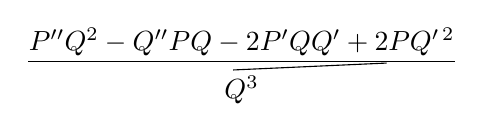
\begin{tikzpicture}
\node[inner sep=0pt,anchor=south west] (num) at (0,0)
 {$P''Q^2-Q''PQ-\unsure{2}P'QQ'+2PQ'^{\,2}$};
\path (num.south west)--(num.south east) coordinate[pos=0.48] (partialstart);
\path (num.south west)--(num.south east) coordinate[pos=0.84] (partialend);
\draw ([yshift=-2pt]num.south west)--([yshift=-2pt]num.south east);
\draw ([yshift=-5pt]partialstart)--([yshift=-2.5pt]partialend);
\node[inner sep=0pt,anchor=north,yshift=-7pt] at (num.south) {$Q^3$};
\end{tikzpicture}}
% The small quotient's fraction rule turns back at its right end; no arrow meaning is assigned.
\figure{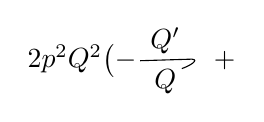
\begin{tikzpicture}
\node[inner sep=0pt,anchor=base west] (prefix) at (0,0) {$2p^2Q^2\bigl(-$};
\node[inner sep=0pt,anchor=south] at ([xshift=0.36cm,yshift=0.08cm]prefix.east) {$Q'$};
\node[inner sep=0pt,anchor=north] at ([xshift=0.36cm,yshift=-0.10cm]prefix.east) {$Q$};
\draw ([xshift=0.04cm]prefix.east)--([xshift=0.70cm,yshift=0.02cm]prefix.east)
 .. controls ([xshift=0.80cm,yshift=0.01cm]prefix.east) and ([xshift=0.66cm,yshift=-0.07cm]prefix.east)
 .. ([xshift=0.57cm,yshift=-0.10cm]prefix.east);
\node[inner sep=0pt,anchor=west] at ([xshift=0.97cm]prefix.east) {$+$};
\end{tikzpicture}}

% Opposite-direction writing, read after a half-turn. Two long diagonals cancel this layer.
\[
\deleted{\det\begin{pmatrix}a\deleted{\unsure{d|b}}&c\\b&d\end{pmatrix}-ad-bc\quad\text{inversible}}
\]
\[
\deleted{\begin{array}{c@{}l}
\delta(e_1 e_{d-2})&=-e_1\delta(e_{d-2})=-e_1e_{d-3}\deleted{=e_d}\\
\rotatebox{90}{$=$}&\\
\delta(a\eta)&=a\delta\eta=a\alpha e_{d-2}+a\beta f_{d-2}
\end{array}}
\]
\[
\deleted{\begin{array}{c@{}l}
\delta(e_1 f_{d-2})&=-\deleted{f}e_1\cdot f_{d-3}\\
\rotatebox{90}{$=$}&\\
b\alpha e_{d-2}+b\beta f_{d-2}&
\end{array}}
\]
\[
\deleted{\begin{array}{c@{}l}
\delta(f_1 e_{d-2})&=\delta(f_1)e_{d-2}-f_1\delta(e_{d-2})=e_{d-2}-f_1e_{d-3}\\
\rotatebox{90}{$=$}&\\
\delta(c\eta)&=c\delta\eta=c\alpha e_{d-2}+c\beta f_{d-2}
\end{array}}
\]
\deleted{etc}

% Detached dot at full-scan x=965--973, y=598--607, below and left of On after rotation.
% Its hand, layer, role, and cancellation state are unresolved; no relation to the formula is assigned.
\(\underset{\unsure{\text{.}}}{\phantom{\text{On}}}\)\deleted{On en tire $e_1e_{d-3}$, $\deleted{f}e_1f_{d-3}$\unsure{,} $f_1e_{d-3}$, $f_1f_{d-3}$ comme comb. lin des $e_{d-1}$ et $f_{d-2}$, à coeff entiers fonctions de $\alpha,\beta$, $a,b,c,d$}

\[
\deleted{\begin{array}{c@{}l}
\delta(e_1x_i)&=-e_1\delta(x_i)=-e_1\deleted{\unsure{\delta}}x_{i-1}\qquad 2\leq i\leq{}\\
\rotatebox{90}{$=$}&\\
\delta(\deleted{\unsure{S}}s e_{i+1}+t f_{i+1})&=s e_i+t f_i
\end{array}}
\]
% archive sheet number: 5

\scanpage{7}
\deleted{\illegible{1}} Soit $a\in\mathbb N^*,b\in\mathbb N^*,c\in\mathbb N^*,\ q\in\mathbb N^*$ \quad $q$ nombre premier $(q\ne1)$

On suppose que $a\mathrel{\underset{1}{\smile}}b$, $a\mathrel{\underset{1}{\smile}}c$, $b\mathrel{\underset{1}{\smile}}c$ (premiers entre eux deux à deux)
\inserted{et $a^q+b^q=c^q$}

On a $c>a$ et $c>b$ car $a\in\mathbb N^*$ et $b\in\mathbb N^*$

On pose $c=a+b'=b+a'$ avec $b'\in\mathbb N^*$ et $a'\in\mathbb N^*$
\[
\begin{aligned}
\text{alors}\qquad a^q+b^q=c^q&=(a+b')^q=\sum_{i=0}^{q}C_q^i\,a^i b'^{\,q-i}\qquad\text{(Newton)}\\
 &=b'^{\,q}+\sum_{i=1}^{q-1}C_q^i\,a^i b'^{\,q-i}+a^q\qquad(\text{car }q\geqslant2)
\end{aligned}
\]
\[
\text{donc}\qquad b^q=\sum_{i=1}^{q-1}C_q^i\,a^i b'^{\,q-i}+b'^{\,q}\tag*{(1)}
\]
la puissance de $b'$ n'étant jamais nulle on peut mettre $b'$ en facteur dans le second membre de (1), donc $b'\mid b^q$ ($b'$ divise $b^q$)

Soit $p$ un nombre premier % The phrase is visibly drawn once by rlap. The phantom preserves its deletion
% annotation and text dimensions without adding the generic horizontal rule.
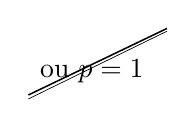
\begin{tikzpicture}[baseline=(cancelled.base)]
\node[inner sep=0pt,outer sep=0pt] (cancelled)
 {\rlap{ou $p=1$}\phantom{\deleted{ou $p=1$}}};
\draw[line width=.55pt] ([xshift=-1.5mm,yshift=-1.5mm]cancelled.south west) -- ([xshift=3mm,yshift=4mm]cancelled.north east);
\draw[line width=.25pt] ([xshift=-1.5mm,yshift=-2mm]cancelled.south west) -- ([xshift=3mm,yshift=3.65mm]cancelled.north east);
\end{tikzpicture}
 et tel que : $p\mid b'$ donc $p\mid b$. Soit $\alpha\in\mathbb N^*$ et $\alpha'\in\mathbb N^*$ tels que
\[
\begin{aligned}
 &p^{\alpha'}\mid b'\quad\text{et}\quad p^{\alpha'+1}\nmid b'\\
 \text{et}\quad &p^\alpha\mid b\quad\text{et}\quad p^{\alpha+1}\nmid b
\end{aligned}
\]
\margin{$\unsure{a|\alpha}$ \unsure{n'exist|n'existe} pas si on avait $p=1$}
On a $\alpha'\leqslant q\alpha$ car $b'\mid b^q$

\[
\begin{aligned}
(1)\ \Longrightarrow\quad&p^{q\alpha}\mid\sum_{i=1}^{q-1}C_q^i\,a^i b'^{\,q-i}+b'^{\,q}\\
\Longrightarrow\quad&p^{q\alpha}\mid b'\left(\sum_{i=1}^{q-1}C_q^i\,a^i b'^{\,q-i-1}+b'^{\,q-1}\right)\qquad(\text{car }q\geqslant2)
\end{aligned}
\]
posons $b'=p^{\alpha'}b''$ donc $b''\mathrel{\underset{1}{\smile}}p$ (propriété de $\alpha'$)
\[
\begin{aligned}
\Longrightarrow\quad&p^{q\alpha}\mid p^{\alpha'}b''\left(\sum_{i=1}^{q-1}C_q^i\,a^i b'^{\,q-i-1}+b'^{\,q-1}\right)\\
\Longrightarrow\quad&p^{q\alpha-\alpha'}\mid b''\left(\sum_{i=1}^{q-1}C_q^i\,a^i b'^{\,q-i-1}+b'^{\,q-1}\right)\quad\text{car }q\alpha\geqslant\alpha'\\
\Longrightarrow\quad&p^{q\alpha-\alpha'}\mid\sum_{i=1}^{q-1}C_q^i\,a^i b'^{\,q-i-1}+b'^{\,q-1}\quad\text{car }b''\mathrel{\underset{1}{\smile}}p
\end{aligned}
\]
% archive sheet number: 6

\scanpage{8}
% Upper-right mottled trace: visible patches only; no character, hand or role assigned.
\margin{
\begin{tikzpicture}[x=1cm,y=1cm]
\draw[gray,line width=.7pt] (.10,.84) -- (.29,.83) -- (.34,.78);
\fill[gray] (.08,.84) circle(.028cm);
\draw[gray,line width=.5pt] (.37,.70) -- (.38,.63) -- (.43,.56);
\draw[gray,line width=.45pt] (.20,.65) -- (.21,.59);
\draw[gray,line width=.45pt] (.27,.50) .. controls(.32,.45) and(.40,.46) .. (.43,.49);
\draw[gray,line width=.65pt] (.13,.31) .. controls(.19,.42) and(.29,.43) .. (.36,.40);
\fill[gray] (.43,.12) circle(.023cm);
\draw[gray,line width=.4pt] (.43,.12) .. controls(.48,.14) and(.49,.19) .. (.48,.23);
\end{tikzpicture}}
Supposons que $q\alpha-\alpha'\ne0$ alors
\[
\begin{aligned}
(1)\ \Longrightarrow\quad &p\mid\sum_{i=1}^{q-1}C_q^i\,a^i b'^{\,q-i-1}+b'^{\,q-1}\\
\Longrightarrow\quad &p\mid q\,a^{q-1}\qquad\text{Car }p\mid b'\ \text{et pour }i\ne q-1\quad q-i-1\deleted{\ne0}>0
\end{aligned}
\]
or $p\mid b'$ et $b'\mid b^q$ donc $b'\mathrel{\underset{1}{\smile}}a$ donc $p\mathrel{\underset{1}{\smile}}a$

\deleted{donc si $\unsure{p\ne1|p\ne q}$}
\[
(1)\ \Longrightarrow\quad p\mid q\qquad\text{donc }\deleted{p=1\ \text{ou }}p=q\quad(\text{si }q\alpha-\alpha'\ne0)
\]
Donc si $p\ne q$ \quad
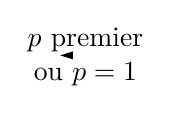
\begin{tikzpicture}[baseline=(p.base)]
\node[inner sep=0pt] (p) at (0,0) {$p$ premier};
\node[inner sep=0pt,anchor=north] at (0,-.28) {\inserted{ou $p=1$}};
% Small dark triangular mark above the addition; its guiding function is uncertain.
\fill (-.32,-.20) -- (-.16,-.15) -- (-.16,-.25) -- cycle;
\end{tikzpicture}
et $p\mid b'$ alors $\alpha'=q\alpha$
\begin{flushright}
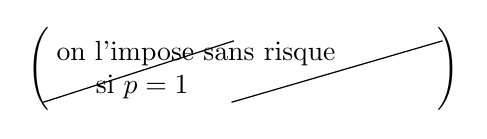
\begin{tikzpicture}[baseline=(u.base)]
\node[inner sep=0pt,anchor=west] (u) at (.22,0)
 {\rlap{on l'impose sans risque}\phantom{\deleted{on l'impose sans risque}}};
\node[inner sep=0pt,anchor=west] (v) at (.72,-.42)
 {\rlap{si $p=1$}\phantom{\deleted{si $p=1$}}};
\node[inner sep=0pt] at (0,-.20)
 {\rlap{$\Bigg($}\phantom{\deleted{$\Bigg($}}};
\node[inner sep=0pt] at (5.2,-.20)
 {\rlap{$\Bigg)$}\phantom{\deleted{$\Bigg)$}}};
% Two separate oblique cancellations over the two-line parenthesis.
\draw[line width=.45pt] (.06,-.62) -- (2.48,.16);
\draw[line width=.45pt] (2.45,-.62) -- (5.13,.16);
\end{tikzpicture}
\end{flushright}

Donc $\exists\,b_0\in\mathbb N^*$ et $\exists\,\gamma\in\mathbb N$ tel que $b'=q^\gamma b_0^q$ \margin{$q\nmid b_0$}

de plus $b_0\mid b$ et si $b=b_0 b''$ alors $b_0\mathrel{\underset{1}{\smile}}b''$ ?

De même $\exists\,a_0\in\mathbb N^*$ et $\exists\,\unsure{\zeta|\delta}\in\mathbb N$ tel que $a'=q^\zeta a_0^q$ avec $a_0\mid a$ et si $\overset{\unsure{\cdot|\prime}}{a}=a_0a''$ alors $a_0\mathrel{\underset{1}{\smile}}a''$ ?

or $a\mathrel{\underset{1}{\smile}}b\Longrightarrow a_{\deleted{\unsure{0}}}'\mathrel{\underset{1}{\smile}}b'\Longrightarrow\zeta\times\gamma=0$ (et aussi $a_0\mathrel{\underset{1}{\smile}}b_0$)

Je suppose désormais que $\zeta=0$ donc $a'=a_0^q$

\figure{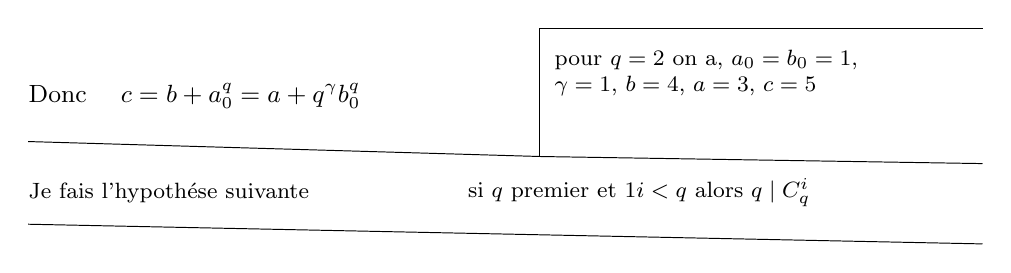
\begin{tikzpicture}[x=1cm,y=1cm]
\node[anchor=west,inner sep=0pt,font=\small] at (0,.80)
 {Donc \quad $c=b+a_0^q=a+q^\gamma b_0^q$};
\node[anchor=north west,inner sep=0pt,font=\footnotesize] at (6.68,1.43)
 {\begin{tabular}{@{}l@{}}
 pour $q=2$ on a, $a_0=b_0=1$,\\
 $\gamma=1$, $b=4$, $a=3$, $c=5$
 \end{tabular}};
% Open right border; the left edge meets the shared long upper rule.
\draw[line width=.35pt] (12.12,1.66) -- (6.50,1.66) -- (6.50,.03);
\draw[line width=.35pt] (0,.22) -- (6.50,.03) -- (12.12,-.06);
\node[anchor=west,inner sep=0pt,font=\footnotesize] at (0,-.43)
 {Je fais l'hypothése suivante};
\node[anchor=west,inner sep=0pt,font=\footnotesize] at (5.58,-.43)
 {si $q$ premier et $1\leqslant i<q$ alors $q\mid C_q^i$};
\draw[line width=.35pt] (0,-.83) -- (12.12,-1.08);
\end{tikzpicture}}
alors Si $q\geqslant3$ et $q\alpha-\alpha'\geqslant2$ \deleted{\unsure{alors}} on a \inserted{$p=q,\ {\unsure{a|\alpha}}'=\gamma$}
\[
\begin{aligned}
(1)\ \Longrightarrow\quad
 &\deleted{\unsure{p^{2}|p}}q^2\mid q\,a^{q-1}\quad
 
\begin{tikzpicture}[baseline=(d.base)]
 \node[inner sep=0pt] (d) at (0,0)
  {\rlap{ou $p=1$}\phantom{\deleted{ou $p=1$}}};
 \draw[line width=.45pt] (d.west) -- (d.east)
  .. controls +(0.22,-.04) and +(0.22,-.06) ..
  ([yshift=-2pt]d.east) -- ([yshift=-2pt]d.west);
 \end{tikzpicture}
\quad
% Faint residual strokes and points in the interline gap; no character is supplied.
\begin{tikzpicture}[baseline=-.05cm,x=1cm,y=1cm]
\draw[gray,line width=.35pt] (0,.12) .. controls (.10,.02) and (.18,-.02) .. (.31,.02);
\draw[gray,line width=.35pt] (.21,.13) -- (.27,.10);
\draw[gray,line width=.35pt] (.34,.02) .. controls (.40,.17) and (.42,.26) .. (.52,.24);
\draw[gray,line width=.35pt] (.49,.15) -- (.64,.14);
\fill[gray] (.58,.31) circle (.5pt);
\fill[gray] (.64,.04) circle (.45pt);
\fill[gray] (.69,-.02) circle (.45pt);
\end{tikzpicture}\\[.8ex]
\Longrightarrow\quad
 &q\mid a^{q-1}\quad
 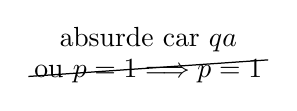
\begin{tikzpicture}[baseline=(d.base)]
 \node[inner sep=0pt] (d) at (0,0)
  {\rlap{ou $p=1\Longrightarrow p=1$}\phantom{\deleted{ou $p=1\Longrightarrow p=1$}}};
 \draw[line width=.45pt] ([xshift=-2pt,yshift=-2pt]d.west)
  -- ([xshift=2pt,yshift=4pt]d.east);
 \node[inner sep=0pt,anchor=south] at (0,.23)
  {\inserted{absurde car $q\nmid a$}};
 \end{tikzpicture}
\end{aligned}
\]
Donc $\gamma=0$ ou $\gamma=$
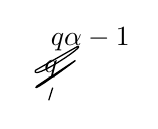
\begin{tikzpicture}[baseline=(q.base)]
\node[inner sep=0pt] (q) at (0,0)
 {\rlap{$q$}\phantom{\deleted{$q$}}};
% The live entry is physically raised above and to the right of the cancelled q.
\node[inner sep=0pt,anchor=south west] at (-.01,.22) {$q\alpha-1$};
\draw[line width=.45pt] (-.20,-.02) -- (.33,.28)
 .. controls (.48,.32) and (-.26,-.17) .. (-.20,-.02);
\draw[line width=.45pt] (-.18,-.22) -- (.30,.10)
 .. controls (.39,.16) and (-.29,-.34) .. (-.18,-.22);
\draw[line width=.45pt] (.02,-.24) -- (-.03,-.40);
\end{tikzpicture}
(sous réserve que l'hypothése est vraie)%
\margin{\begin{tikzpicture}[baseline=(n.base)]
\node[inner sep=0pt,text width=.85\marginparwidth] (n)
 {C'est peut-être interessant car ici $2$ est mis à part dans
 \(\mathord{\overset{\scriptscriptstyle\unsure{/}}{\vphantom{l}}}\)l'ensemble des nombres premiers};
% Small detached rising stroke before l'ensemble: role and hand unresolved.
% Return arrow rises at the right from the final parenthesis toward this note.
\fill ([xshift=.07cm,yshift=-.47cm]n.south east) circle(.022cm);
\draw ([xshift=.15cm,yshift=-.47cm]n.south east) -- ([xshift=.31cm,yshift=-.47cm]n.south east)
 -- ([xshift=.35cm,yshift=-.16cm]n.north east)
 .. controls([xshift=.35cm,yshift=-.03cm]n.north east) and([xshift=.19cm,yshift=-.01cm]n.north east)
 .. ([xshift=.06cm,yshift=.01cm]n.north east);
\draw ([xshift=.19cm,yshift=.14cm]n.north east) .. controls([xshift=.00cm,yshift=.04cm]n.north east) and([xshift=-.01cm,yshift=-.06cm]n.north east) .. ([xshift=.15cm,yshift=-.10cm]n.north east);
\end{tikzpicture}}
% archive sheet number: 7

\scanpage{10}
% Consolidated by root from three independent readings and seventeen adjudication crops.
% crop-candidate: scan 10
\figure{%
\begin{tikzpicture}[x=.0056cm,y=-.0056cm,line cap=round,line join=round,line width=.57pt,
 every node/.style={font=\scriptsize,inner sep=1pt}]
% Upper row. Coordinates follow the scans, with y increasing toward the foot.
\draw (118,180) .. controls (96,175) and (65,165) .. (63,146) .. controls (60,125) and (74,98) .. (94,68) .. controls (114,54) and (139,53) .. (158,62) .. controls (185,75) and (200,102) .. (186,137) .. controls (174,168) and (147,184) .. (118,180) -- cycle;
\draw (80,83) .. controls (88,71) and (96,67) .. (99,65);
\draw (136,55) .. controls (127,87) and (124,146) .. (117,181);
\draw (318,164) .. controls (303,149) and (280,133) .. (288,110) .. controls (294,84) and (305,65) .. (324,65) .. controls (344,61) and (369,61) .. (385,78) .. controls (402,97) and (402,127) .. (387,146) .. controls (369,166) and (333,176) .. (318,164) -- cycle;
\draw (304,85)--(313,65) (292,83) .. controls (303,69) and (310,78) .. (316,72);
\draw (359,63) .. controls (347,100) and (337,144) .. (319,163);
\draw (386,75) .. controls (376,99) and (355,139) .. (359,165);
\draw (528,88) .. controls (548,68) and (579,74) .. (590,94) .. controls (606,122) and (591,152) .. (572,164) .. controls (549,174) and (523,169) .. (512,155) .. controls (495,128) and (504,101) .. (528,88) -- cycle;
\draw (505,107) .. controls (512,94) and (526,94) .. (530,85);
\draw (527,88) -- (544,125) -- (563,157);
\draw (512,158) -- (544,125) -- (579,82);
\fill (545,125) circle[radius=7.5];
\node at (568,39) {OK};
\draw (714,165) .. controls (692,138) and (707,102) .. (741,82) .. controls (763,71) and (805,69) .. (824,85) .. controls (845,101) and (838,140) .. (811,169) .. controls (783,190) and (740,190) .. (714,165) -- cycle;
\draw (750,82) .. controls (741,112) and (733,154) .. (716,171);
\draw (789,74) .. controls (771,116) and (760,159) .. (758,188);
\draw (821,83) .. controls (812,113) and (798,150) .. (809,171);
\draw (774,82) -- (788,74);
\draw (877,167) .. controls (874,143) and (884,111) .. (899,102) .. controls (914,94) and (943,93) .. (957,104) .. controls (971,119) and (978,145) .. (968,163) .. controls (951,183) and (921,193) .. (898,188) .. controls (882,184) and (875,177) .. (877,167) -- cycle;
\draw (899,101) .. controls (909,128) and (902,148) .. (877,166);
\draw (934,99) .. controls (946,117) and (947,134) .. (977,137);
\draw (898,186) .. controls (925,163) and (946,151) .. (968,162);
\draw (925,98)--(927,104) (934,98)--(940,106);
\draw (1007,168) .. controls (1007,137) and (1016,107) .. (1031,102) .. controls (1052,96) and (1065,106) .. (1066,128) .. controls (1065,157) and (1048,186) .. (1027,195) .. controls (1016,201) and (1009,184) .. (1007,168) -- cycle;
\draw (1015,118) -- (1031,130) -- (1063,132) (1008,170) -- (1032,129) -- (1057,103);
\draw (1015,194) .. controls (1031,167) and (1054,156) .. (1054,176);
\fill (1033,130) circle[radius=5.3];
\draw (1038,111)--(1055,103);
\draw (1089,170) .. controls (1094,140) and (1114,106) .. (1137,93) .. controls (1161,77) and (1199,88) .. (1222,101) .. controls (1246,124) and (1228,161) .. (1207,184) .. controls (1180,207) and (1144,214) .. (1121,202) .. controls (1102,193) and (1091,184) .. (1089,170) -- cycle;
\draw (1086,171) -- (1137,135) -- (1167,113) -- (1196,92);
\draw (1119,103) -- (1138,135) .. controls (1151,149) and (1170,178) .. (1184,195);
\draw (1156,86) .. controls (1161,103) and (1168,122) .. (1179,137) .. controls (1195,152) and (1201,165) .. (1217,172);
\draw[line width=3pt] (1138,135) -- (1167,113);
\node at (1153,55) {OK};
\draw (1306,198) .. controls (1298,178) and (1312,140) .. (1333,113) .. controls (1351,93) and (1383,82) .. (1400,89) .. controls (1420,98) and (1435,120) .. (1430,147) .. controls (1413,188) and (1379,216) .. (1344,216) .. controls (1326,214) and (1312,207) .. (1306,198) -- cycle;
\draw (1317,195)--(1397,89) (1328,115)--(1425,174) (1297,172) .. controls (1340,167) and (1385,161) .. (1436,139);
\fill (1338,166)--(1363,135)--(1394,153)--cycle;
\draw[line width=2pt] (1376,90) .. controls (1385,86) and (1397,86) .. (1404,94);
\node at (1376,52) {OK};
\draw (1490,75) .. controls (1477,75) and (1450,148) .. (1446,194) .. controls (1442,229) and (1454,246) .. (1486,240);
\node at (1495,165) {ou};
\draw (1554,177) .. controls (1552,150) and (1562,112) .. (1579,106) .. controls (1599,99) and (1624,111) .. (1633,135) .. controls (1642,163) and (1621,194) .. (1600,205) .. controls (1579,218) and (1555,209) .. (1554,177) -- cycle;
\draw (1566,129) .. controls (1578,149) and (1590,162) .. (1618,175);
\draw (1583,104) .. controls (1582,132) and (1587,174) .. (1597,205);
\draw (1568,206)--(1613,107);
\draw (1567,184) .. controls (1567,196) and (1567,206) .. (1571,209);
\draw[line width=1pt] (1592,178) .. controls (1591,196) and (1590,217) .. (1587,238);
\fill (1587,159) circle[radius=6.5];
% Detached dark fragments beside the lower descending stroke; role uncertain.
\draw[line width=.7pt] (1596,174)--(1595,180) (1595,182)--(1593,187);
\fill (1584,198) circle[radius=1.2]; \fill (1598,226) circle[radius=1.2];
\draw[opacity=.45] (1548,116) .. controls (1562,103) and (1574,101) .. (1584,102);
\draw (1632,96) .. controls (1647,66) and (1657,114) .. (1649,157) .. controls (1641,212) and (1624,259) .. (1606,273);
\draw (759,202) .. controls (780,226) and (799,220) .. (828,212) .. controls (843,208) and (846,205) .. (846,217) .. controls (872,197) and (918,220) .. (949,210) -- (944,207);
\draw[line width=.55pt] (746,274) .. controls (747,244) and (777,229) .. (821,226) .. controls (863,222) and (910,214) .. (923,230) .. controls (940,253) and (888,293) .. (840,300) .. controls (787,310) and (751,304) .. (746,282) -- cycle;
\draw[line width=.7pt] (949,271) .. controls (947,245) and (987,240) .. (1015,235) .. controls (1044,226) and (1072,217) .. (1068,255) .. controls (1064,295) and (1053,303) .. (1014,305) .. controls (969,310) and (951,299) .. (949,271) -- cycle;
\node[inner sep=0pt] at (121,235) {\begin{minipage}{75pt}
\diagram{\begin{tikzcd}[ampersand replacement=\&,column sep=4pt,row sep=0pt,cells={nodes={inner sep=0pt,outer sep=0pt}}]
\bullet
\end{tikzcd}}
\end{minipage}};
\node[inner sep=0pt] at (325,236) {\begin{minipage}{75pt}
\diagram{\begin{tikzcd}[ampersand replacement=\&,column sep=4.7pt,row sep=0pt,cells={nodes={inner sep=0pt,outer sep=0pt}}]
\bullet \& \bullet
\end{tikzcd}}
\end{minipage}};
\node[inner sep=0pt] at (533,233) {\begin{minipage}{75pt}
\diagram{\begin{tikzcd}[ampersand replacement=\&,column sep=13pt,row sep=0pt,cells={nodes={inner sep=0pt,outer sep=0pt}}]
\vphantom{\bullet}\arrow[r,dash,line width=.65pt,start anchor=center,end anchor=center,shorten <=1pt,shorten >=1pt] \& \vphantom{\bullet}
\end{tikzcd}}
\end{minipage}};
\node[inner sep=0pt] at (852,253) {\begin{minipage}{75pt}
\diagram{\begin{tikzcd}[ampersand replacement=\&,column sep=8pt,row sep=0pt,cells={nodes={inner sep=0pt,outer sep=0pt}}]
\bullet \& \bullet \& \bullet
\end{tikzcd}}
\end{minipage}};
\node[inner sep=0pt] at (1009,262) {\begin{minipage}{75pt}
\diagram{\begin{tikzcd}[ampersand replacement=\&,column sep=4pt,row sep=0pt,cells={nodes={inner sep=0pt,outer sep=0pt}}]
\vphantom{\bullet}\arrow[r,dash,line width=.65pt,start anchor=center,end anchor=center,shorten <=1pt,shorten >=1pt] \&[5.2pt] \vphantom{\bullet} \&[-2pt] \bullet
\end{tikzcd}}
\end{minipage}};
\node[inner sep=0pt] at (1152,251) {\begin{minipage}{75pt}
\diagram{\begin{tikzcd}[ampersand replacement=\&,column sep=8.3pt,row sep=0pt,cells={nodes={inner sep=0pt,outer sep=0pt}}]
\bullet\arrow[r,dash,line width=.65pt,start anchor=center,end anchor=center,shorten <=1pt,shorten >=1pt] \& \unsure{\bullet|\circ}\arrow[r,dash,line width=.65pt,start anchor=center,end anchor=center,shorten <=2.7pt,shorten >=1pt] \& \bullet
\end{tikzcd}}
\end{minipage}};
\node[inner sep=0pt] at (1326,262) {\begin{minipage}{75pt}
\diagram{\begin{tikzcd}[ampersand replacement=\&,column sep=1.2pt,row sep=2.0pt,cells={nodes={inner sep=0pt,outer sep=0pt}}]
{} \& \bullet\arrow[dl,dash,line width=.65pt]\arrow[dr,dash,line width=.65pt] \& {}\\
\bullet\arrow[rr,dash,line width=.65pt] \& {} \& \bullet
\end{tikzcd}}
\end{minipage}};
% Two small, detached ink traces near the upper edge.
% Detached upper-edge marks: their hand and function remain undetermined.
\draw[opacity=.65,line width=.55pt] (1018,26) .. controls (1020,31) and (1023,32) .. (1025,27);
\draw[opacity=.65,line width=.55pt] (1037,29)--(1037,26) .. controls (1040,28) and (1043,28) .. (1046,25)--(1046,28);
% Middle row, left group.
\draw (116,390) .. controls (129,357) and (164,337) .. (200,327) .. controls (226,322) and (254,320) .. (272,326) .. controls (307,338) and (328,377) .. (326,413) .. controls (324,455) and (301,485) .. (265,500) .. controls (239,512) and (207,515) .. (184,510) .. controls (147,506) and (125,480) .. (116,455) .. controls (111,433) and (112,411) .. (116,390) -- cycle;
\draw (122,399) .. controls (122,392) and (126,388) .. (131,388);
\draw (154,353) .. controls (158,379) and (146,454) .. (128,472);
\draw (205,327) .. controls (203,354) and (205,404) .. (201,431) .. controls (197,465) and (193,491) .. (191,513);
\draw (270,324) .. controls (258,366) and (252,404) .. (253,433) .. controls (252,456) and (256,486) .. (263,501);
\draw (311,367) .. controls (296,393) and (290,441) .. (305,475);
\draw[opacity=.2] (192,503)--(195,556);
\draw (400,505) .. controls (378,492) and (374,467) .. (377,444) .. controls (382,413) and (403,377) .. (420,364) .. controls (441,342) and (462,334) .. (482,340) .. controls (514,337) and (544,366) .. (542,403) .. controls (543,444) and (508,491) .. (484,503) .. controls (462,516) and (428,521) .. (400,505) -- cycle;
\draw (419,365) .. controls (426,377) and (409,469) .. (400,503);
\draw (482,343) .. controls (461,390) and (451,446) .. (449,510);
\draw (517,356) .. controls (502,397) and (484,451) .. (481,501);
\draw[line width=1.6pt] (406,503) .. controls (423,481) and (428,504) .. (433,517);
\draw (433,512)--(434,519) (448,491)--(447,513) (456,346)--(482,340);
\draw (568,459) .. controls (563,432) and (570,399) .. (581,379) .. controls (594,358) and (612,345) .. (640,352) .. controls (665,358) and (685,385) .. (687,411) .. controls (693,446) and (680,490) .. (647,519) .. controls (636,523) and (624,523) .. (609,524) .. controls (590,517) and (571,499) .. (568,480) -- cycle;
\draw (598,359) .. controls (613,387) and (599,433) .. (567,459);
\draw (645,353) .. controls (653,386) and (676,407) .. (693,410);
\draw (570,480) .. controls (590,487) and (605,503) .. (610,524);
\draw[line width=1pt] (644,519) .. controls (647,504) and (665,473) .. (682,462);
\draw[line width=1.8pt] (684,395) .. controls (697,432) and (683,488) .. (651,516);
\draw (178,557) .. controls (177,574) and (221,577) .. (266,570) .. controls (311,564) and (361,554) .. (376,584) .. controls (378,560) and (416,560) .. (439,563) .. controls (497,573) and (539,558) .. (631,549);
\fill (733,427) circle[radius=2]; \fill (713,443) circle[radius=1.1];
% Middle row, right group.
\draw (778,444) .. controls (795,393) and (841,368) .. (889,367) .. controls (926,365) and (959,385) .. (977,414) .. controls (1001,449) and (966,489) .. (944,514) .. controls (923,544) and (901,563) .. (874,562) .. controls (842,564) and (800,553) .. (774,526) .. controls (774,509) and (771,472) .. (778,444) -- cycle;
\draw (772,446) .. controls (815,439) and (889,422) .. (947,388);
\draw (790,536) -- (854,425) -- (891,367);
\draw (778,464) .. controls (801,466) and (800,495) .. (777,509);
\draw (909,368) .. controls (910,392) and (925,388) .. (937,375);
\draw (774,517) .. controls (783,516) and (781,535) .. (791,536);
\fill (855,425) circle[radius=7.6];
\draw (990,500) .. controls (989,465) and (1002,432) .. (1026,409) .. controls (1047,386) and (1072,381) .. (1088,394) .. controls (1114,409) and (1110,444) .. (1104,473) .. controls (1098,508) and (1073,550) .. (1052,568) .. controls (1023,582) and (1009,571) .. (1000,548) .. controls (994,529) and (990,511) .. (990,500) -- cycle;
\draw (1021,412) .. controls (1043,438) and (1062,481) .. (1078,517);
\draw (998,534) .. controls (1023,505) and (1065,431) .. (1091,399);
\draw (998,456) .. controls (1018,463) and (1009,490) .. (991,501);
\draw (1015,570) .. controls (1034,544) and (1052,547) .. (1057,562);
\fill (1053,458) ellipse[x radius=6.8,y radius=9];
\draw (1133,512) .. controls (1136,476) and (1157,427) .. (1183,402) .. controls (1209,376) and (1248,380) .. (1268,395) .. controls (1296,420) and (1293,459) .. (1285,493) .. controls (1274,530) and (1241,562) .. (1208,571) .. controls (1171,582) and (1146,555) .. (1137,534) .. controls (1133,523) and (1132,516) .. (1133,512) -- cycle;
\draw (1172,411) -- (1207,472) .. controls (1222,498) and (1233,526) .. (1243,551);
\draw (1144,552) .. controls (1161,534) and (1218,450) .. (1266,395);
\draw (1155,453) .. controls (1175,478) and (1159,506) .. (1133,523);
\draw (1159,444) .. controls (1166,453) and (1181,440) .. (1171,428);
\fill (1207,472) circle[radius=7.3];
\draw (1285,514) .. controls (1291,476) and (1311,437) .. (1337,415) .. controls (1356,400) and (1381,409) .. (1391,423) .. controls (1417,463) and (1404,507) .. (1384,535) .. controls (1369,559) and (1349,583) .. (1327,588) .. controls (1306,591) and (1288,575) .. (1284,550) .. controls (1281,536) and (1282,525) .. (1285,514) -- cycle;
\draw (1315,444) -- (1342,491) -- (1368,559);
\draw (1290,564) .. controls (1307,552) and (1355,466) .. (1388,423);
\draw (1299,575) .. controls (1317,554) and (1335,524) .. (1347,555) -- (1353,570);
\draw (1312,585) .. controls (1328,561) and (1340,561) .. (1340,582);
\fill (1343,492) circle[radius=6.6];
\fill (1307,505) .. controls (1310,497) and (1314,496) .. (1318,483) .. controls (1324,477) and (1329,500) .. (1324,509) .. controls (1317,520) and (1305,515) .. (1307,505) -- cycle;
% Undetermined trace: pale intervals separate the darker parts of this upper extension.
\draw[opacity=.22] (1328,433) .. controls (1330,406) and (1335,357) .. (1341,329);
\draw[line width=.65pt] (1340,332)--(1339,339) (1338,343) .. controls (1336,351) and (1337,359) .. (1335,365);
\draw[line width=.55pt] (1333,382)--(1332,389) (1331,398)--(1330,403) (1329,411)--(1327,432);
\draw[line width=1.8pt] (1327,436) .. controls (1335,425) and (1340,416) .. (1349,418);
\draw (793,583) .. controls (822,621) and (923,616) .. (981,613) .. controls (1025,612) and (1060,623) .. (1079,622) .. controls (1090,628) and (1095,637) .. (1102,649) .. controls (1114,632) and (1127,626) .. (1138,621) .. controls (1220,627) and (1280,619) .. (1348,616) .. controls (1354,610) and (1360,601) .. (1364,592);
\draw (1004,605) .. controls (1015,626) and (1050,615) .. (1069,622) (1167,622) -- (1204,630);
\node[font=\bfseries\small] at (539,658) {?};
\node[inner sep=0pt] at (373,646) {\begin{minipage}{85pt}
\diagram{\begin{tikzcd}[ampersand replacement=\&,column sep=7pt,row sep=0pt,cells={nodes={inner sep=0pt,outer sep=0pt}}]
\bullet \& \bullet \& \bullet \& \bullet
\end{tikzcd}}
\end{minipage}};
\node[inner sep=0pt] at (848,648) {\begin{minipage}{85pt}
\diagram{\begin{tikzcd}[ampersand replacement=\&,column sep=11.1pt,row sep=0pt,cells={nodes={inner sep=0pt,outer sep=0pt}}]
\vphantom{\bullet}\arrow[r,dash,line width=.65pt,start anchor=center,end anchor=center,shorten <=1pt,shorten >=1pt] \& \vphantom{\bullet} \& \bullet \& \bullet
\end{tikzcd}}
\end{minipage}};
% Lower row.
\draw[opacity=.22,line width=.4pt] (1518,375) .. controls (1540,374) and (1561,405) .. (1524,401);
\fill[opacity=.75] (1566,580) circle[radius=1.25]; \fill[opacity=.65] (1561,587) circle[radius=1];
\node at (201,691) {OK};
\draw (123,811) .. controls (135,770) and (168,740) .. (208,726) .. controls (239,716) and (275,725) .. (304,749) .. controls (339,775) and (354,809) .. (350,840) .. controls (347,879) and (314,935) .. (279,960) .. controls (257,972) and (226,969) .. (198,968) .. controls (162,965) and (130,943) .. (121,913) .. controls (114,887) and (118,844) .. (123,811) -- cycle;
\draw (124,893) .. controls (149,863) and (184,800) .. (219,718);
\draw (125,813) -- (194,773) .. controls (223,757) and (257,743) .. (274,727);
\draw (198,968) -- (298,838) -- (340,790);
\draw (277,965) .. controls (283,927) and (291,876) .. (298,839) .. controls (303,812) and (307,781) .. (310,754);
\fill (194,773) circle[radius=7.5]; \fill (299,838) circle[radius=7];
\draw[opacity=.14] (252,825)--(256,825) (259,825)--(264,826) (267,826)--(271,826) (274,827)--(278,827);
\draw[opacity=.4] (278,827)--(293,828);
% State remains uncertain: diagonal cancellation | hatching. Only the visible diagonal paths are inked.
\node[inner sep=0pt,outer sep=0pt,anchor=center] at (548,820) {\unsure{\rlap{\hbox{\begin{tikzpicture}[x=.0056cm,y=-.0056cm,line cap=round,line join=round,line width=.57pt,color=black]
\path[use as bounding box] (450,714) rectangle (646,926);
\draw (460,830) .. controls (473,785) and (509,749) .. (541,731) .. controls (566,724) and (595,741) .. (613,754) .. controls (645,781) and (638,817) .. (626,842) .. controls (605,883) and (571,914) .. (538,917) .. controls (508,924) and (480,912) .. (462,889) .. controls (452,874) and (454,848) .. (460,830) -- cycle;
\draw (474,789) -- (612,754) (461,891) -- (547,729) (556,729) .. controls (578,778) and (605,805) .. (628,838);
% Repeated diagonal cancellation strokes in this disk.
\draw (535,717) .. controls (526,729) and (457,833) .. (461,835) .. controls (470,838) and (538,725) .. (537,729) .. controls (515,764) and (465,860) .. (470,865) .. controls (476,870) and (554,747) .. (565,747) .. controls (549,777) and (493,861) .. (493,865) .. controls (504,870) and (569,753) .. (585,751) .. controls (557,783) and (513,860) .. (518,866) .. controls (526,877) and (601,791) .. (614,798) .. controls (618,801) and (589,843) .. (563,892) .. controls (554,907) and (560,914) .. (572,923);
% Small pale descending trace and dark tip at the lower-left outline.
\draw[opacity=.16,line width=.4pt] (490,861) .. controls (488,885) and (490,901) .. (491,915);
\draw[line width=.55pt] (491,912)--(490,920);
\end{tikzpicture}}}\phantom{\deleted{\hbox{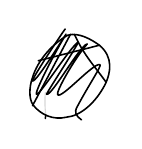
\begin{tikzpicture}[x=.0056cm,y=-.0056cm,line cap=round,line join=round,line width=.57pt,color=black]
\path[use as bounding box] (450,714) rectangle (646,926);
\draw (460,830) .. controls (473,785) and (509,749) .. (541,731) .. controls (566,724) and (595,741) .. (613,754) .. controls (645,781) and (638,817) .. (626,842) .. controls (605,883) and (571,914) .. (538,917) .. controls (508,924) and (480,912) .. (462,889) .. controls (452,874) and (454,848) .. (460,830) -- cycle;
\draw (474,789) -- (612,754) (461,891) -- (547,729) (556,729) .. controls (578,778) and (605,805) .. (628,838);
% Repeated diagonal cancellation strokes in this disk.
\draw (535,717) .. controls (526,729) and (457,833) .. (461,835) .. controls (470,838) and (538,725) .. (537,729) .. controls (515,764) and (465,860) .. (470,865) .. controls (476,870) and (554,747) .. (565,747) .. controls (549,777) and (493,861) .. (493,865) .. controls (504,870) and (569,753) .. (585,751) .. controls (557,783) and (513,860) .. (518,866) .. controls (526,877) and (601,791) .. (614,798) .. controls (618,801) and (589,843) .. (563,892) .. controls (554,907) and (560,914) .. (572,923);
% Small pale descending trace and dark tip at the lower-left outline.
\draw[opacity=.16,line width=.4pt] (490,861) .. controls (488,885) and (490,901) .. (491,915);
\draw[line width=.55pt] (491,912)--(490,920);
\end{tikzpicture}}}}}};
\draw (666,836) .. controls (669,808) and (686,789) .. (706,785) .. controls (725,782) and (746,786) .. (755,803) .. controls (773,824) and (771,857) .. (758,880) .. controls (746,903) and (728,917) .. (706,910) .. controls (683,903) and (660,871) .. (666,836) -- cycle;
\draw (707,786) -- (694,902) (747,789) .. controls (739,827) and (735,869) .. (729,906);
\draw (666,840)--(767,844);
\draw[line width=3.4pt] (699,838)--(737,842);
\draw (718,786) .. controls (715,814) and (733,813) .. (737,789);
\draw (797,850) .. controls (804,822) and (821,801) .. (839,798) .. controls (864,797) and (876,815) .. (881,839) .. controls (890,866) and (876,895) .. (860,910) .. controls (841,926) and (822,917) .. (809,905) .. controls (796,890) and (792,870) .. (797,850) -- cycle;
\draw (827,805) .. controls (823,843) and (819,878) .. (816,915);
\draw (862,805) .. controls (858,842) and (854,879) .. (852,914);
\draw (799,861)--(890,859); \draw[line width=2.8pt] (820,857)--(853,857);
\draw (874,818) .. controls (868,841) and (868,848) .. (885,850);
\draw (543,948) .. controls (573,976) and (607,963) .. (665,954) .. controls (706,949) and (731,945) .. (741,967) .. controls (744,947) and (789,945) .. (826,944) .. controls (864,943) and (881,941) .. (899,937) -- (898,931);
\node at (1156,724) {OK};
\draw (1004,849) .. controls (1005,815) and (1033,783) .. (1069,769) .. controls (1101,757) and (1134,762) .. (1150,787) .. controls (1172,815) and (1183,855) .. (1165,903) .. controls (1149,943) and (1125,964) .. (1109,969) .. controls (1072,976) and (1040,970) .. (1024,945) .. controls (1004,913) and (997,879) .. (1004,849) -- cycle;
\draw[opacity=.65] (1006,850) .. controls (1002,859) and (1003,869) .. (1009,874);
\draw (1012,924) .. controls (1029,875) and (1050,817) .. (1070,770);
\draw (1011,808) .. controls (1055,804) and (1125,796) .. (1156,788);
\draw (1101,764) .. controls (1110,780) and (1116,791) .. (1120,798) -- (1174,881);
\draw (1109,967) .. controls (1127,926) and (1154,855) .. (1172,823);
\draw[line width=2.7pt] (1056,802)--(1119,794);
\draw[line width=3.7pt] (1118,795)--(1158,853);
% Detached short dark trace below the broad segment; role and hand undetermined.
\draw[line width=.55pt] (1166,875)--(1165,879);
% Detached pale irregular patch; hand, origin and role remain undetermined.
\filldraw[fill opacity=.10,draw opacity=.16,line width=.3pt]
(1629,793) .. controls (1629,790) and (1631,788) .. (1635,788)
--(1636,786)--(1640,790)--(1645,792)
.. controls (1649,795) and (1648,799) .. (1646,802)
--(1643,803)--(1640,806)--(1637,808)--(1634,804)--(1630,804)
.. controls (1627,801) and (1627,797) .. (1629,793)--cycle;
% Two faint, angular lines at the foot, crossing the last graph and continuing at the right.
\draw[opacity=.55] (1010,975) .. controls (1027,995) and (1035,1030) .. (1044,1050) .. controls (1053,1074) and (1061,1090) .. (1075,1089);
\draw[line width=1.5pt] (1041,1036) .. controls (1052,1070) and (1060,1090) .. (1074,1088);
\draw[opacity=.16] (1073,1088) .. controls (1108,1087) and (1162,1076) .. (1214,1064) -- (1288,985);
\draw[opacity=.5] (1215,1073)--(1237,1044) (1246,1033)--(1261,1014) (1278,996)--(1289,982);
\draw[opacity=.22] (1345,934) .. controls (1353,954) and (1350,994) .. (1358,1009) -- (1372,1014);
\draw[line width=1.9pt] (1373,1014) .. controls (1390,1025) and (1430,1037) .. (1458,1048) -- (1484,1054) -- (1500,1036);
\draw[opacity=.5] (1487,1054)--(1581,957);
\draw[opacity=.23] (1568,905) .. controls (1572,924) and (1571,943) .. (1581,957);
\node[inner sep=0pt] at (222,1035) {\begin{minipage}{94pt}
\diagram{\begin{tikzcd}[ampersand replacement=\&,column sep=5.2pt,row sep=0pt,cells={nodes={inner sep=0pt,outer sep=0pt}}]
\unsure{\circ|\bullet}\arrow[r,dash,line width=.65pt,start anchor=center,end anchor=center,shorten <=1pt,shorten >=1pt] \& \circ \& \hspace{3.3pt} \& \bullet\arrow[r,dash,line width=.65pt,start anchor=center,end anchor=center,shorten <=1pt,shorten >=1pt] \& \bullet
\end{tikzcd}}
\end{minipage}};
\node[inner sep=0pt] at (563,1026) {\begin{minipage}{94pt}
\diagram{\begin{tikzcd}[ampersand replacement=\&,column sep=7pt,row sep=0pt,cells={nodes={inner sep=0pt,outer sep=0pt}}]
\unsure{\circ|\bullet}\arrow[r,dash,line width=.65pt,start anchor=center,end anchor=center,shorten <=1pt,shorten >=1pt] \& \bullet\arrow[r,dash,line width=.65pt,start anchor=center,end anchor=center,shorten <=2.7pt,shorten >=1pt] \& \bullet \& \bullet
\end{tikzcd}}
\end{minipage}};
\node[inner sep=0pt] at (1075,1032) {\begin{minipage}{94pt}
\diagram{\begin{tikzcd}[ampersand replacement=\&,column sep=9pt,row sep=0pt,cells={nodes={inner sep=0pt,outer sep=0pt}}]
\unsure{\bullet|\circ}\arrow[r,dash,line width=.65pt,start anchor=center,end anchor=center,shorten <=1pt,shorten >=1pt] \& \bullet\arrow[r,dash,line width=.65pt,start anchor=center,end anchor=center,shorten <=1pt,shorten >=1pt] \& \bullet\arrow[r,dash,line width=.65pt,start anchor=center,end anchor=center,shorten <=1pt,shorten >=1pt] \& \bullet
\end{tikzcd}}
\end{minipage}};

% Hook projecting above/right of the uncertain middle vertex under upper disk 7.
\draw[line width=.65pt] (1153,251) .. controls (1154,245) and (1159,246) .. (1163,252);
% Tiny detached spot just above the outer lower arch in the last middle disk.
\fill (1314,543) circle[radius=1.4];
% Pale detached marks; hand, purpose, and surface origin remain undetermined.
% Above upper disk4 the short course is supported; its faint lower continuation is unresolved.
\draw[opacity=.14,line width=.4pt] (416,241) .. controls (425,250) and (426,260) .. (421,266) .. controls (416,274) and (410,275) .. (403,275);
\draw[opacity=.16,line width=.4pt] (784,42) .. controls (784,49) and (785,55) .. (787,62);
\draw[opacity=.4,line width=.4pt] (786,56)--(786,59);
\draw[opacity=.16,line width=.35pt] (369,743) .. controls (379,751) and (390,762) .. (405,778) -- (415,786);
\draw[opacity=.25,line width=.4pt] (377,751)--(384,758) (390,764)--(393,767);
\draw[opacity=.14,line width=.4pt] (1567,352) .. controls (1570,358) and (1576,360) .. (1580,362);
% Pale diagonal inside the right angular trace, with independently detached lower dash.
% Only the short supported course is reproduced; a farther upper continuation remains unresolved.
\node[anchor=north west,inner sep=0pt,outer sep=0pt] at (1438,978) {\unsure{\hbox{\begin{tikzpicture}[x=.0056cm,y=-.0056cm,line cap=round,color=black]
\path[use as bounding box] (1438,978) rectangle (1504,1039);
\draw[opacity=.13,line width=.4pt] (1444,1037) .. controls (1460,1018) and (1488,989) .. (1500,980);
\end{tikzpicture}}}};
\draw[opacity=.45,line width=.45pt] (1435,1084)--(1437,1093);
% Dark pieces and small detached marks around the upper-right angular-trace endpoint.
\draw[opacity=.75,line width=.45pt] (1568,908)--(1570,917);
\fill[opacity=.65] (1566,921) circle[radius=1.15];
\fill[opacity=.3] (1550,893) circle[radius=1.2];
\fill[opacity=.2] (1603,930) circle[radius=1.6];
\end{tikzpicture}}
% archive sheet number: 9

\scanpage{11}
\[
 \unsure{=|\Rightarrow}
\]
\[
 \begin{aligned}
 \mathbb P\left(
 \begin{tikzpicture}[x=.0043cm,y=-.0043cm,baseline={(0,82)},line cap=round,line join=round]
 \draw[line width=.5pt] (18,12) -- (59,76) (64,1) -- (23,78);
 \draw[line width=.5pt] (0,1) -- (30,3) (63,0) -- (76,1)
 (0,80) -- (26,78) (58,76) -- (78,77);
 \end{tikzpicture}\right)&\qquad
 P(X\times\unsure{Z|2})\overset{?}{\simeq}
 \operatorname{Hom}(\underset{\unsure{\cdot}}{\deleted{\unsure{e|\mathcal E}}Z}\times X,\mathscr E)\\
 &\qquad\mathrel{/\!/}\quad
 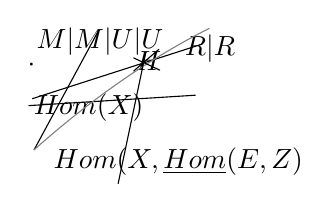
\begin{tikzpicture}[x=.011cm,y=-.011cm,baseline=(live.base),line cap=round,line join=round]
 % The cancellation paths are drawn explicitly. Invisible deleted copies retain the deletion annotation.
 \node[anchor=base west,inner sep=0] at (74,110)
 {\rlap{$\operatorname{Hom}(X)$}\phantom{$\deleted{\operatorname{Hom}(X)}$}};
 \node[inner sep=0] at (151,26)
 {$\unsure{\rlap{$M$}\phantom{\deleted{M}}|M|\rlap{$U$}\phantom{\deleted{U}}|U}$};
 \node[inner sep=0] at (207,48)
 {\rlap{$H$}\phantom{$\deleted{H}$}};
 \node[inner sep=0] at (278,34)
 {$\unsure{\rlap{$R$}\phantom{\deleted{R}}|R}$};
 \draw (69,100) -- (261,88);
 \draw (73,92) -- (269,29);
 \draw (75,151) -- (149,14);
 \draw[gray] (75,151) .. controls (120,111) and (191,54) .. (277,11);
 \draw (172,190) -- (204,38);
 \draw (190,60) -- (219,35) (190,45) -- (220,59);
 \node[inner sep=0] at (72,54) {$\unsure{\cdot}$};
 \node[anchor=base west,inner sep=0] (live) at (97,173)
 {$\operatorname{Hom}(X,\underline{\operatorname{Hom}}(\mathscr E,Z)$};
 \end{tikzpicture}\\
 \unsure{O|0}\subset\mathbb{P}(X)&\qquad
 \operatorname{Hom}(\mathscr E,\underline{\operatorname{Hom}}(X,Z))\\
 &\qquad\mathrel{/\!/}\\
 &\qquad P(\operatorname{Hom}(X,Z)
 \end{aligned}
\]
\figure{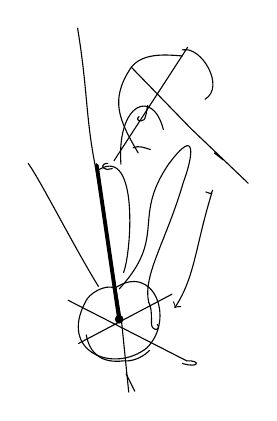
\begin{tikzpicture}[x=.011cm,y=-.011cm,line cap=round,line join=round]
\draw (63,1) .. controls (75,74) and (72,104) .. (84,163) -- (114,342) -- (122,421);
\draw[line width=1.4pt] (85,159) -- (111,337);
\draw (6,157) .. controls (22,180) and (57,250) .. (87,299);
\draw (64,365) -- (172,308) (52,315) -- (189,385);
\draw (106,301) .. controls (151,271) and (176,337) .. (143,370)
 .. controls (105,400) and (41,375) .. (72,317) .. controls (76,307) and (95,296) .. (106,301);
\fill (111,337) circle (5);
\draw (105,154) -- (190,23) (184,26) .. controls (206,21) and (234,69) .. (210,83)
 (125,46) -- (194,117) -- (260,180) (231,153) -- (221,145);
\draw (133,145) .. controls (110,106) and (100,83) .. (125,46) .. controls (139,28) and (169,32) .. (184,33);
\draw (113,158) .. controls (108,87) and (150,70) .. (162,118);
\draw (88,164) .. controls (134,137) and (125,261) .. (116,283);
\draw (111,302) .. controls (167,241) and (125,221) .. (168,158)
 .. controls (202,112) and (196,150) .. (185,179) .. controls (166,245) and (138,286) .. (145,317);
\draw[->] (218,191) .. controls (199,252) and (199,287) .. (175,324);
% Local small paths seen in the junction and disk crops; no letter or role assigned.
\draw (98,157) .. controls (90,157) and (90,163) .. (97,164) -- (103,163);
\draw (127,139) .. controls (134,136) and (140,139) .. (147,141);
\draw (144,90) .. controls (142,98) and (142,109) .. (136,108)
 .. controls (132,108) and (131,105) .. (134,103);
\draw (73,355) .. controls (77,377) and (91,388) .. (116,385)
 .. controls (128,386) and (139,380) .. (146,373);
\draw (189,385) .. controls (205,384) and (204,394) .. (184,388);
\draw (145,317) .. controls (151,329) and (146,344) .. (150,347)
 .. controls (156,352) and (158,345) .. (155,343);
\draw (119,400) -- (129,420);
\draw (211,190) -- (217,192) -- (219,188);
% crop-candidate: scan 11
\end{tikzpicture}}
\[
 \begin{aligned}
 \begin{tikzpicture}[baseline=(hom.base),line cap=round]
 \node[inner sep=0] (hom) at (0,0) {$\underline{\operatorname{Hom}}$};
 \node[inner sep=0] at (-.78,.12) {\unsure{\begin{tikzpicture}[x=.015cm,y=-.015cm]
 \draw[gray] (0,0) .. controls (3,3) and (6,5) .. (10,6);
 \draw (10,6) -- (12,6.5);
 \end{tikzpicture}}};
 \end{tikzpicture}(X,Y)&\subset P(X\times Y)\\
 \operatorname{Hom}(\begin{tikzpicture}[baseline=(z.base),line cap=round,line join=round]
 \node[inner sep=0] (z) at (0,0) {$\deleted{\unsure{t|1}}Z$};
 \node[inner sep=0] at (.17,.48) {\unsure{\begin{tikzpicture}[line cap=round,line join=round]
 \draw (0,0) -- (.08,.06) -- (.15,.03) -- (.23,.06) -- (.30,.04);
 \fill (.38,.04) circle (.012);
 \fill[gray] (.43,.03) circle (.009);
 \end{tikzpicture}}};
 \end{tikzpicture}\times X,Y)&\subset
 \underset{\text{\unsure{\begin{tikzpicture}[x=.014cm,y=-.014cm,baseline=0,line cap=round,line join=round]
 \draw (-13,0) -- (-8,1);
 \draw (-2,2) -- (0,-2) -- (3,1) -- (5,-1) -- (6,2);
 \draw (10,-1) -- (11,3);
 \end{tikzpicture}}}}{P}
 (\underset{\text{\unsure{\begin{tikzpicture}[x=.014cm,y=-.014cm,baseline=0,line cap=round]
 \fill (-8,0) circle (1.2);
 \fill[gray] (1,1) circle (1.4);
 \draw[gray] (6,2) -- (8,-1) (12,1) -- (13,-1) (15,0) -- (17,-2);
 \end{tikzpicture}}}}{Z}\times X\times Y)
 \end{aligned}
\]
\diagram{\begin{tikzcd}[ampersand replacement=\&,row sep=small,column sep=small,
 execute at end picture={
  % Retraced lower horizontal arrow shaft and extended upper head stroke.
  \draw[line width=.45pt] ([xshift=-4pt,yshift=-1pt]sxiU.west)
    .. controls ([xshift=-18pt,yshift=-5pt]sxiU.west) and ([xshift=15pt,yshift=-5pt]sxiV.east)
    .. ([xshift=4pt,yshift=-1pt]sxiV.east);
  \draw ([xshift=8pt,yshift=5pt]sxiV.east) -- ([xshift=11pt,yshift=9pt]sxiV.east);
  % Loop at the downward arrowhead, plus its two detached marks.
  \draw ([xshift=-5pt,yshift=9pt]sxiPX.north)
    .. controls ([xshift=-9pt,yshift=14pt]sxiPX.north) and ([xshift=-10pt,yshift=8pt]sxiPX.north)
    .. ([xshift=-4pt,yshift=6pt]sxiPX.north);
  \node[inner sep=0] at ([xshift=-12pt,yshift=14pt]sxiPX.north) {$\unsure{\cdot}$};
  \node[inner sep=0] at ([xshift=14pt,yshift=5pt]sxiPX.north) {$\unsure{\textcolor{gray}{\cdot}}$};
 }]
 \& {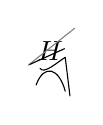
\begin{tikzpicture}[baseline=(h.base),line cap=round,line join=round]
 \node[inner sep=0] (h) at (0,0) {\rlap{$H$}\phantom{$\deleted{H}$}};
 \draw[gray] (-.28,-.18) -- (.31,.29);
 \draw (-.26,-.17) -- (.18,.03);
 \draw (-.13,-.22) .. controls (-.08,-.30) and (.09,-.14) .. (.19,-.08);
 \draw (.19,-.08) -- (.25,-.57);
 \draw (-.18,-.43) .. controls (-.08,-.16) and (.11,-.21) .. (.19,-.51);
 \end{tikzpicture}} \& \& \\
 \& {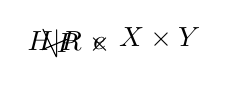
\begin{tikzpicture}[baseline=(prod.base),line cap=round,line join=round]
 \node[inner sep=0] at (-.12,0) {\rlap{$\unsure{H|R}$}\phantom{$\deleted{\unsure{H|R}}$}};
 \node[inner sep=0] (prod) at (.04,0) {$P$};
 \draw (-.27,.18) -- (-.10,-.17) (-.28,-.08) -- (.03,.05);
 \node[inner sep=0] at (.45,0) {\rlap{$e$}\phantom{$\deleted{e}$}};
 \node[inner sep=0] at (.45,-.02) {$\times$};
 \node[anchor=base west,inner sep=0] at (.69,-.04) {$X\times Y$};
 \end{tikzpicture}}
 \arrow[d,"{
\begin{tikzpicture}[baseline=(u.base),line cap=round,line join=round]
 \node[inner sep=0] (u) at (0,0)
 {\rlap{$\unsure{H|U}$}\phantom{$\deleted{\unsure{H|U}}$}};
 \draw (-.21,-.21) -- (.24,.36);
 \draw (.05,-.13) .. controls (-.03,-.45) and (.13,-.54) .. (.33,-.31);
 \end{tikzpicture}}"'] \& \&
 {\supset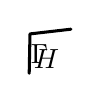
\begin{tikzpicture}[baseline=(g.base),line cap=round,line join=round]
 \node[inner sep=0] at (.09,-.04) {\rlap{$H$}\phantom{$\deleted{H}$}};
 \node[inner sep=0] (g) at (0,.03) {$\Gamma$};
 \draw[line width=1.1pt] (-.13,-.22) -- (-.12,.28) -- (.40,.34);
 \end{tikzpicture}}\arrow[dll] \\
 \& |[alias=sxiPX]| P\times X\arrow[dl] \& \& U\times_{\unsure{Y|V}}U\\
 {\begin{tikzpicture}[baseline=(p.base),line cap=round]
 \node[inner sep=0] (p) at (.29,-.25) {$P$};
 \node[inner sep=0] at (-1.03,.91) {$\unsure{\cdot}$};
 \draw[gray] (-1.11,.94) .. controls (-1.10,.92) and (-1.08,.91) .. (-1.07,.90);
 \draw (-.08,1.0) .. controls (-.06,.35) and (-.12,-.55) .. (-.09,-1.04);
 \draw (-.06,.48) .. controls (-.03,-.10) and (.02,-.67) .. (.08,-.92);
 \node[inner sep=0] at (.21,.03) {\unsure{\begin{tikzpicture}[x=.015cm,y=-.015cm,line cap=round]
 \draw[gray] (0,0) .. controls (3,-3) and (4,0) .. (3,3) -- (4,8);
 \end{tikzpicture}}};
 \end{tikzpicture}}
 \& |[alias=sxiV]| \unsure{V|W} \& \& |[alias=sxiU]| U\arrow[ll]\\
 \& \& {\begin{tikzpicture}[x=.011cm,y=-.011cm,baseline=(p.base),line cap=round]
 \node[inner sep=0,anchor=base] (p) at (0,0) {$P$};
 \draw (-42,-102) .. controls (-30,-94) and (-30,-78) .. (-22,-66);
 \draw[gray] (60,-113) -- (30,-59);
 \fill (30,-59) circle (1.2);
 \node[inner sep=0] at (2,21) {\unsure{\begin{tikzpicture}[x=.011cm,y=-.011cm,line cap=round]
 \draw[line width=.7pt] (-1,-13) .. controls (0,-4) and (1,5) .. (3,13);
 \fill (3,13) circle (1.2);
 \end{tikzpicture}}};
 \end{tikzpicture}} \&
\end{tikzcd}}
\figure{\begin{tikzpicture}[x=.011cm,y=-.011cm,line join=round,line cap=round]
% crop-candidate: scan 11
% The three bottom drawings were checked individually on the supplied halves.
\draw (13,425) -- (98,53);
\draw (98,46) -- (130,35) (139,32) -- (155,26) (164,23) -- (215,4);
\draw (215,4) -- (282,69);
\draw (282,76) -- (267,303) -- (145,352) -- (13,425);
\draw (215,4) -- (210,-3) (219,5) -- (218,-4);
\draw (13,425) -- (6,414) (267,303) -- (270,313);
\draw[line width=1.8pt] (216,8) -- (272,69) (278,226) -- (267,304) -- (147,351) -- (41,253);
\draw (209,4) .. controls (230,40) and (248,53) .. (272,68) (282,74) -- (219,0);
\draw (6,237) .. controls (47,191) and (63,184) .. (74,188)
 (3,214) -- (144,362) -- (178,405) (6,209) -- (159,358);
\draw (35,185) .. controls (-5,206) and (15,266) .. (48,309)
 .. controls (115,383) and (151,428) .. (171,406);
\draw[->] (46,199) .. controls (80,196) and (208,305) .. (184,407);
\draw (86,366) .. controls (86,389) and (188,345) .. (237,329);
\draw (319,271) -- (430,382) -- (549,389) -- (624,258) (319,271) -- (498,464) (535,454) -- (617,264);
\draw[line width=2pt] (325,275) -- (429,374) -- (556,384) -- (620,263);
\draw (319,268) -- (556,384) (361,299) -- (543,381);
\draw (501,486) .. controls (530,446) and (552,450) .. (570,357);
\draw (416,389) .. controls (421,396) and (430,396) .. (438,389);
\draw (562,388) -- (574,391) (564,398) -- (578,402);
\node[inner sep=0] at (523,276) {\unsure{\begin{tikzpicture}[x=.011cm,y=-.011cm,line cap=round]
\fill (0,0) circle (1.2); \draw[gray] (1,1) -- (3,2);
\end{tikzpicture}}};
\draw (627,259) -- (745,421);
\draw (640,291) .. controls (722,169) and (814,239) .. (883,324)
 .. controls (934,419) and (753,461) .. (678,394) .. controls (654,378) and (643,338) .. (648,316);
\draw (676,252) .. controls (710,302) and (679,351) .. (678,400)
 (705,230) .. controls (675,312) and (707,386) .. (709,416)
 (731,225) .. controls (722,312) and (765,383) .. (782,421);
\draw (783,244) -- (868,399) (815,250) .. controls (797,322) and (811,374) .. (850,416)
 (860,285) .. controls (847,342) and (824,363) .. (822,426);
\draw (684,318) -- (698,354) -- (685,337) -- (698,365)
 (811,316) -- (835,347) -- (812,328) -- (837,358) -- (813,342) -- (833,369);
\end{tikzpicture}}
% archive sheet number: 10
